\section{Experiment 1}

The first step of getting clock synchronisation to work, was to figure
out a way to measure the current rate of data sent to the USB device.

A Nucleo-F411RE devboard was used to mock up a USB audio card. 

\todo{Add theory on devboards. Include info on gpios and their
alternate functions}
\todo{Add theory on the different STM32 devboards discussed}

This board can be configured as a Full Speed USB device, which enables a
bandwidth of up to 12 Mbit/s. This is enough bandwidth to transmit two
channels of audio at a sampling rate of 48 kHz.

The goal of experiment 1 was to set up a USB audio class device, and
for each USB interrupt to this device toggle a \acrshort{gpio} pin.
This pin was then connected to a Saleae logic analyzer, which could
record the rate this pin changed.

The changes of the states of these pins where recorded with the logic
analyzer. These recordings where parsed into a diagram of the rate of
interrupts over time, using a python script included in the USB Audio
Experiments repository \cite{github:usbAudioExperiments}.

\begin{figure}[h]
	\caption{Rate over time for experiment 1}
	\centering
	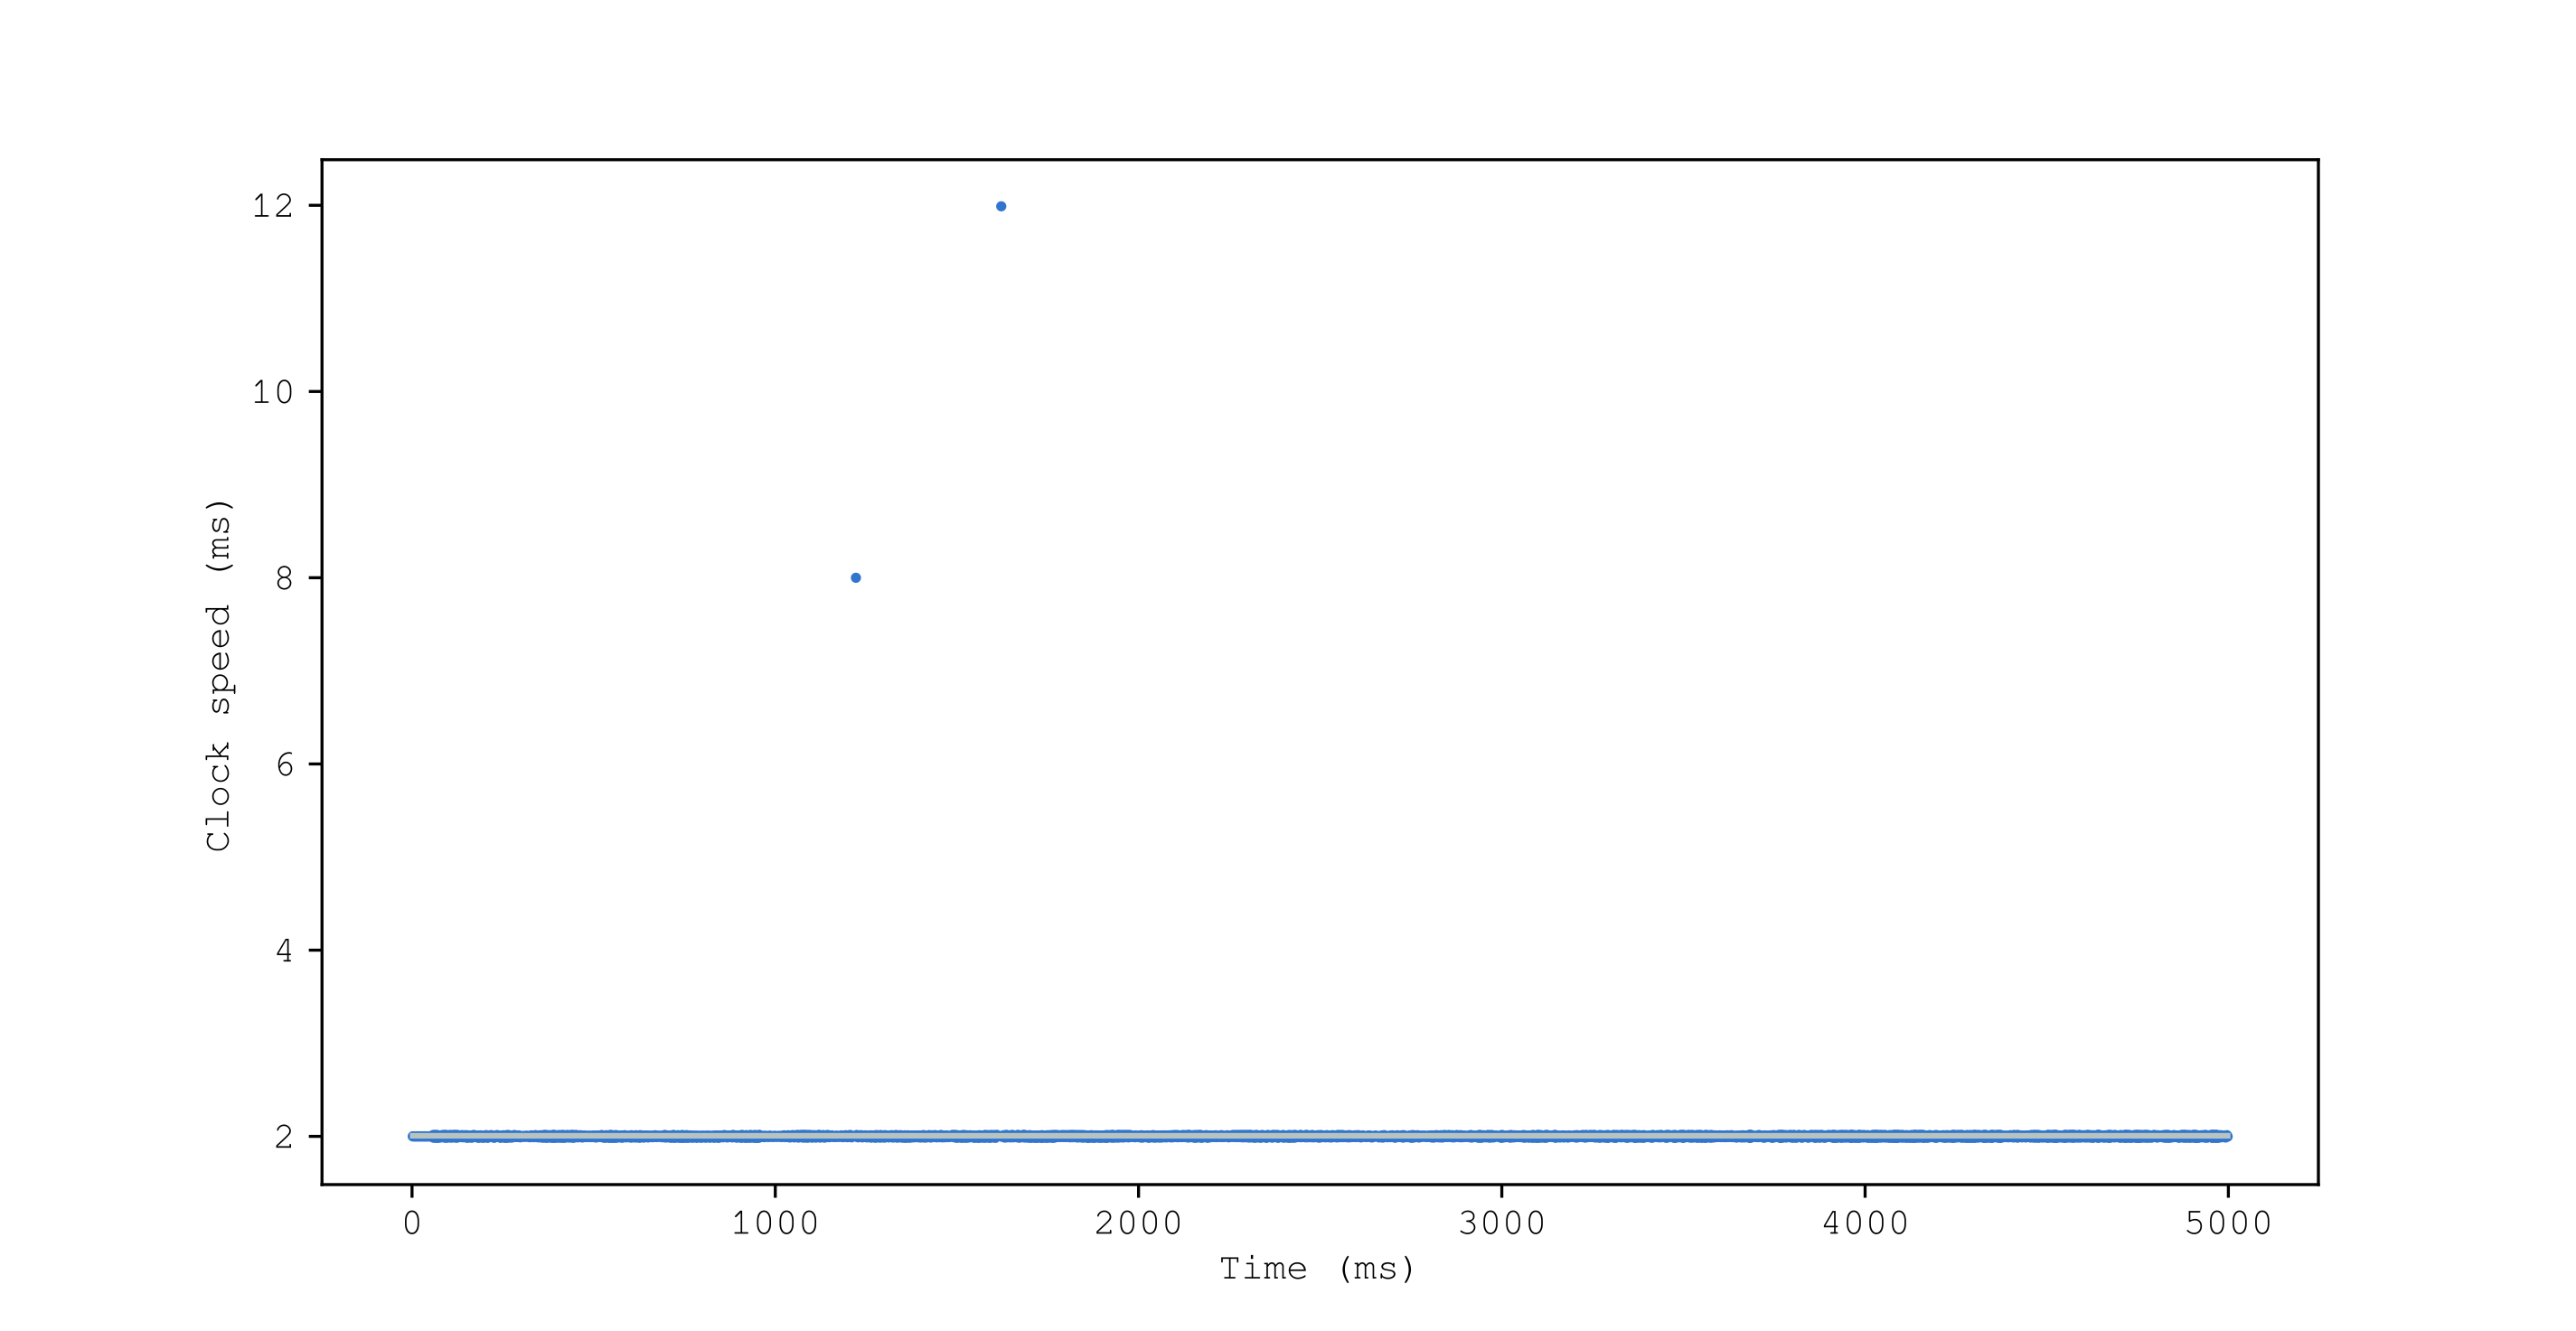
\includegraphics[width=0.8\textwidth]{Experiment-1/Experiment-1.png}
	\label{fig:experiment-1}
\end{figure}

Figure \ref{fig:experiment-1} shows the result for this experiment.
The result is a rate of one USB request every two milliseconds. There
is however two outliers, where one request took eight milliseconds,
and one twelve milliseconds. Figure \ref{fig:experiment-1-raw}
displays Saleaes analyzer software Logic. This includes the normal
rates at about two milliseconds each, and one of the outliers where
packets seems to have been dropped

\begin{figure}[h]
	\caption{A piece of the captured data for experiment 1, in Saleaes
	analyzer software Logic.}
	\centering
	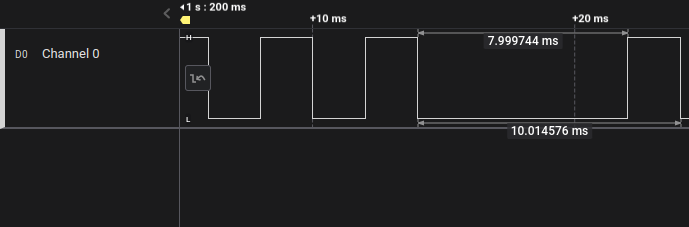
\includegraphics[width=0.8\textwidth]{Experiment-1/Experiment-1-raw.png}
	\label{fig:experiment-1-raw}
\end{figure}

The reason for these outliers might have been caused by the choice of
the USB hosts operating system, which was Ubuntu. It could also depend
on the fact that the host computer acted both as a USB host for the
audio output, the devboard programmer and the logic analyzer at the
same time, which might have limited the bandwidth available for the
audio device, and therefore dropping USB messages. Another cause could
have been that the USB connection between the host machine and the
mocked up audio card was made using patch cables, with an unspecified
impedance, resulting in an unstable USB connection.
